%!TEX root = thesis.tex
\chapter{Data-wise Opportunistic Routing with Spatial Information}
\label{DORSI}
% \SVN $Revision: 838 $
% \SVN $Author: sgordon $
% \SVN $Date: 2014-05-12 13:30:42 +0700 (Mon, 12 May 2014) $
% \SVN $URL: https://sandilands.info/svn/Common/Styles/siitthesis/chapter4.tex $
As for now, the routing algorithms for opportunistic network has been barely concerned about the content of data. 
%%
The routing decision for this type of network is usually based on node topology environment. 
%%
However, there are several data dissemination methods based on the context of data. 
%%
Yazhou et al. \cite{Jiao2009} proposed the data dissemination in DTN based on content classification which classifies the forwarding messages by their content, every node only requests the message that it is interested in. 
%%
This research showed that this method can provide low overhead while maintaining high delivery rate and low delivery latencies compared to epidemic routing. 
%%
While in other content-based network scheme \cite{Carzaniga2004}, message content is structured as a set of attribute/value pairs, and a selection predicate is a logical disjunction of conjunctions of elementary constraints over the values of individual attributes. 
%%
Both techniques differ from DORSI in the sense that they route all messages by sets of rules while our protocol route messages differently depend on their priority class.

A number of related researches attempt to address the main criticism of flooding based routing protocol in term of network congestion. 
%%
APRA \cite{Jin2009} arranges the forwarding sequence and the dropping sequence based on their assigned priority. 
%%
This priority is determined by the TTL, Delivery Predictability, and Replication Density. 
%%
While Joe et al. \cite{Joe2010} developed a DTN message priority routing protocol by modify the spray and wait \cite{Spyropoulos2005} flooding-based routing protocol. 
%%
However, these prioritizing mechanisms aim to rank the messages by defined matrices which involving network topology. 
%%
In contrast, DORSI protocol routes the data based solely on the content of data itself.

Although all of the above mentioned the routing method by the content of message to limit the number of message flooding in the network. The messages traversing in the network are treated the same except containing different attributes. The routing decision depends on the sets of rules and nodes. In this chapter, we propose a new routing technique to assure the deliverable of important data while maintain the lower message replicas. The routing decision depends on the class of data itself. In addition, we improve the overall performance by appending the geographic information for forwarding node selection.

In this chapter, we present a routing protocol in opportunistic environment that dynamically prioritizes the candidate messages based on the content of the data. Since security is an increasing concern in military and other critical operation mission, it is vital to route data of different sensitivities differently. The most significant and sensitive data should be guaranteed its higher level of delivery and protection than common data. However, only few works have applied the well-defined information sensitivity concept such as Multi Level of Security (MLS) \cite{Kotrappa2010,marking2010} to network information such as routing information, QoS signaling and other management information \cite{Winjum2008}.

In this routing scheme, we purpose to incorporate the information sensitivity concept into the messages in order to route the data differently in compliance with the classes of messages. To the best of our knowledge, this method has not been fully explored in the existing literatures. In this research, we extend our previous work \cite{Kerdsri2012} by generalizing information sensitivity parameters and involving spatial information into routing decision to improve the network efficiency. We conducted Opportunistic Network Environment (ONE) simulation \cite{Keranen2009b} to evaluate the performance of DORSI protocol.
%=============================================================================
\section{Opportunistic network model}
\label{DORSI:Opportunistic network model}
%=============================================================================

\begin{figure}[!t]
\centering
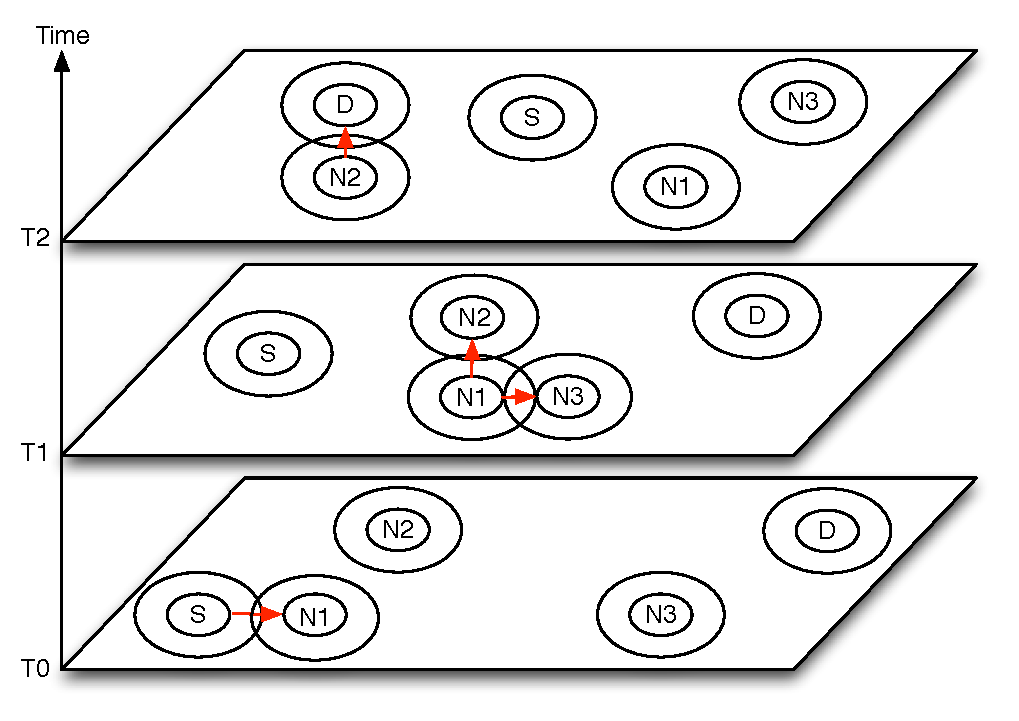
\includegraphics[width=5in]{Figures/OpportunisticNetworkNodel.pdf}
\caption{Opportunistic network model}
\label{Opportunistic network model}
\end{figure}

Since opportunistic network commonly operates in multi-hop wireless ad-hoc network environment, links may be disrupted or shut down periodically when nodes move away or absent which resulting in intermittent connectivity \cite{Moreira2011}. As a result, nodes require to communicate with each other via opportunistic contacts through store - carry - forward fashion \cite{Chung-Ming2008}. Instead of selecting a node to act as the next hop, multiple relay nodes may be determined when a data packet is being transmitted. This decision is carried out for each data packet according to the instantaneous wireless links condition in order to select the best relaying nodes. In OppNet, a node is an entity acting as a host, router or gateway. Each node can route and exchange message (full-duplex) between nodes that move randomly among remote fragment of network within its contact period. Nevertheless, OppNet node must contain enough processing power and storage to keep the data until this node gets contact with intermediate carrier or destination node. Within this disruptive environments, the contact period is extremely dynamic since contact may appear arbitrarily without prior information and this transmission link can be absent at any time.

Fig. \ref{Opportunistic network model} presents the model of OppNet routing exploiting their node mobility and contacts for data delivery. A node can exchange message with other intermediate nodes inside its wireless coverage area until the message reach the destination. From Fig. \ref{Opportunistic network model}, all node can move with time (T0 - T2 as an example). At T0, The source node transmit the data to the next node within its radio coverage. This receptors at T1 now can act as a relay node and replicate message to the other nodes in its wireless link radius until this message reach the final destination at T3. Therefore, OppNet leads to a load balancing while it increases the robustness of the multi-hop wireless network as multiple receptors are potential relays.


%=============================================================================
\section{DORSI routing algorithm}
\label{DORSI:DORSI routing algorithm}
%=============================================================================
\begin{figure}[!t]
\centering
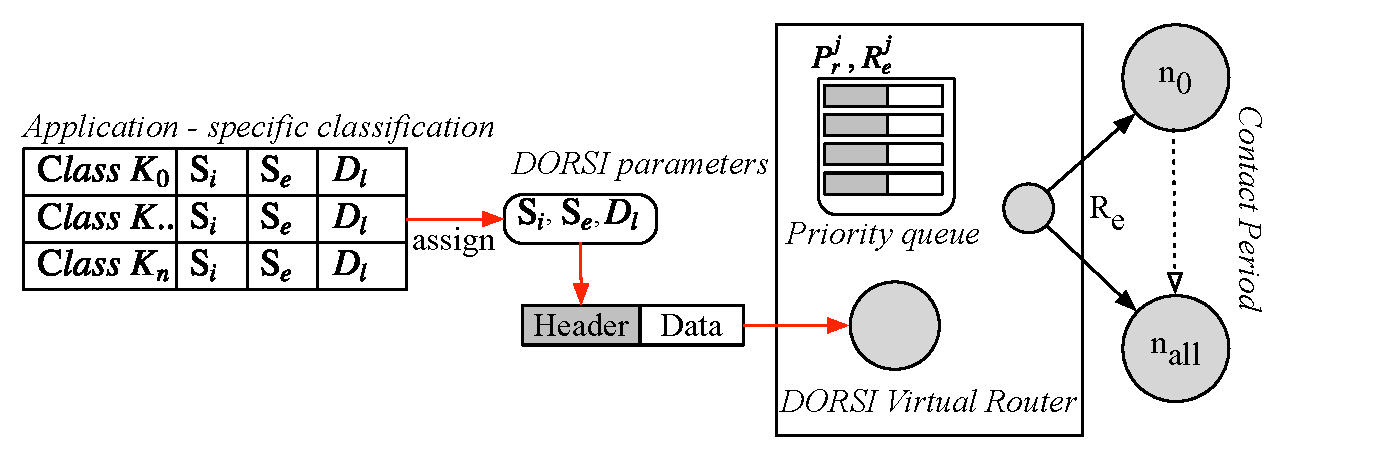
\includegraphics[width=5.5in]{Figures/DORSIsystemModel.pdf}
\caption{DORSI system model}
\label{DORSI system model}
\end{figure}

The design goal of DORSI is to distinguish the data with different information sensitivity concept. 
%%
We implement this protocol in order to guarantee that the important message can reach the destination within the time limit resulting in higher delivery ratio. 
%%
Additionally, we need to control the security risk of the message with higher security level by limiting the number of message replica in this network according with information sensitivity concept \cite{Kotrappa2010,marking2010}. 
%%
The final goal of this protocol is to increase the bandwidth efficiency by selecting the candidate nodes with higher probability of delivering the message to the destination.

Fig. \ref{DORSI system model} shows the proposed DORSI system model implemented as a virtual (software) router in an OppNet node. 
%%
In DORSI, besides common routing information such as source and destination addresses, every delivered message is associated with 3 additional DORSI parameters which are Significant level ($S_i$) Security level ($S_e$), Delivery deadline ($D_l$). 
%%
The $S_i$ represents how important of this message while the $S_e$ defines the level of this data that needs to be protected. 
%%
The $D_l$ element is the message expiration time. 
%%
If the delivery deadline is reached, the message will be dropped. 
%%
The value of these DORSI parameters are determined in accordance with the application specific requirement. 
%%
For example, the contents in military domain are divided into several classifications based on the multilevel of security which is intended to prevent unauthorized personnel from accessing information at higher classification than their authorization \cite{Winjum2008}. 
%%
Therefore, different classes of message in military perspective are treated differently.


At DORSI router, a time-constrained priority queue is used to carry DORSI messages waiting for being forwarded to the next node. 
%%
The DORSI parameters: $S_i$ , $S_e$ and $D_l$ are used in routing decision of DORSI virtual router on a node when this node opportunistically contacts to the other nodes. 
%%
Upon node contact, messages will be processed orderly according to their up-to-date priority value, however the message whose delivery deadline is reached will not be considered and will be removed out of the queue. 
%%
The priority value ($P_r^j$) of a specific message, $j$, is calculated based on its significant level and its expediting factor, $\xi(D_l^j, t)$, as in Eq. \ref{Eq:DORSI:routing algorithm}

\begin{eqnarray}
\label{Eq:DORSI:routing algorithm}
{ P }_{ r }^{ j }={ w }_{ p }{ S }_{ i }^{ j }+(1-{ w }_{ p })\xi ({ D }_{ l }^{ j },t)
\end{eqnarray}

where

\begin{equation*}
 \xi ({ D }_{ l }^{ j },t)=\begin{cases} 0;{ \tau  }_{ t }>{ \tau  }_{ max } \\ \frac { { \tau  }_{ max }-{ \tau  }_{ t } }{ { \tau  }_{ max }-{ \tau  }_{ min } }  \\ 1;{ \tau  }_{ t }<{ \tau  }_{ max } \end{cases};{ \tau  }_{ min }\le { \tau  }_{ t }\le { \tau  }_{ max } 	
\end{equation*}

The $W_p$ level and expediting factor components.
%%
We define $\tau_t$ as residual lifetime of message which is calculated from $D_t^j - t$. 
%%
The expediting factor value, in the range [0,1], is composed from the message
residual lifetime, compared with the maximum and minimum countable message lifetime, $\tau_{max}$ and $\tau_{min}$, in the system. 
%%
The message with the residual lifetime $\tau_t$ = $\tau_{max}$ is considered as no need to expedite the message delivery while the message with $\tau_{min}$ is considered for maximum expediting.
%%
Note that the $P_r^j$ value will be recalculated at every time any node get contacted. 
%%
When a specific message,$j$ , is being processed, the determination whether it should be copied and sent to a specific contact node is controlled by the replication probability value, $R_j^e$, calculated at a contact time as in Eq. \ref{Eq:DORSI:replication probability}.


\begin{eqnarray}
\label{Eq:DORSI:replication probability}
{ R }_{ e }^{ j }=(1-{ R }_{ min })[{ w }_{ r }{ P }_{ r }+(1-{ w }_{ r })(1-{ S }_{ e }^{ j })]+{ R }_{ min }
\end{eqnarray}

The replication probability value, in range of [${ R }_{ min }$, 1], is based on the concept that a message with
more priority, $P_r^j$, should be disseminated more in order to increase delivery ratio while the message with more security level should be replicated less in order to tighten security risk. 
%%
In the formula, the replication weight coefficient, $w_r$ , is used to balance effect between both components. 
%%
The ${ R }_{ min }$ is the minimum guaranteed replication probability value in the system so that even a message with very low priority and very high security still has a chance to be forwarded. 
%%
This ${ R }_{ min }$ is a configurable system parameter according to application requirement.
In case that there are several nodes simultaneously contacts when processing a specific message, the node with higher rank will be considered before the lower one. 
%%
The ranking value of a contacting node, 𝑛, is calculated according to its departure probability representing the relative chance to move away from the DORSI router node, $r$.

\begin{eqnarray}
\label{Eq:DORSI:node ranking model}
{ N }_{ r }^{ n }=\sqrt { { ({ x }_{ n }\cos { { \theta  }_{ n } } -{ x }_{ r }^{ t }\cos { { \theta  }_{ r }^{ t } } ) }^{ 2 }-{ ({ y }_{ n }\sin { { \theta  }_{ n } } -{ x }_{ r }^{ t }\sin { { \theta  }_{ r }^{ t } } ) }^{ 2 } } -\sqrt { { ({ x }_{ n }-{ x }_{ r }^{ t }) }^{ 2 }-{ ({ y }_{ n }-{ x }_{ r }^{ t }) }^{ 2 } } 
\end{eqnarray}

It can be estimated as the difference in distance between the current DORSI router, $r$, and the contacting node $n$ , after they moves further one unit distance in their current direction. 
%%
Given that the positions of the router $r$ and the contacting node $n$ are $(x_r,y_r)$ and $(x_n,y_n)$. 
%%
In addition, their moving direction vectors are 
$\vec { { d }_{ r } } =\cos { { \theta  }_{ r } } \hat { x } +\sin { { \theta  }_{ r } } \hat { y } $
and
$\vec { { d }_{ n } } =\cos { { \theta  }_{ n } } \hat { x } +\sin { { \theta  }_{ n } } \hat { y } $
, respectively. 
%%
The ranking value, $N_{r}^n$ is defined by formula in Eq. \ref{Eq:DORSI:node ranking model}. 
%%
The positive $N_{r}^n$ value means the contacting node is moving away while the negative value means that it becomes closer. 
%%
The contacting node with higher $N_{r}^n$ is needed to be considered since there is higher probability that it will be out of reach soon, compared with the other nodes. 
%%
In Fig. \ref{Eq:DORSI:node ranking model}, $D_0$ represents the distance between node $r$ and $n$ at time $t$ = 0 while $D_1$ is a distance at the time t=1. 
%%
If $D_1 > D_0$ , both nodes tend to move away from each other which results in higher node ranking.
%%
Note that all messages where lifetime reach their deadline are discarded from the carried node. 
%%
In addition, DORSI node will not receive the same copy of a specific message.

\begin{figure}[!t]
\centering
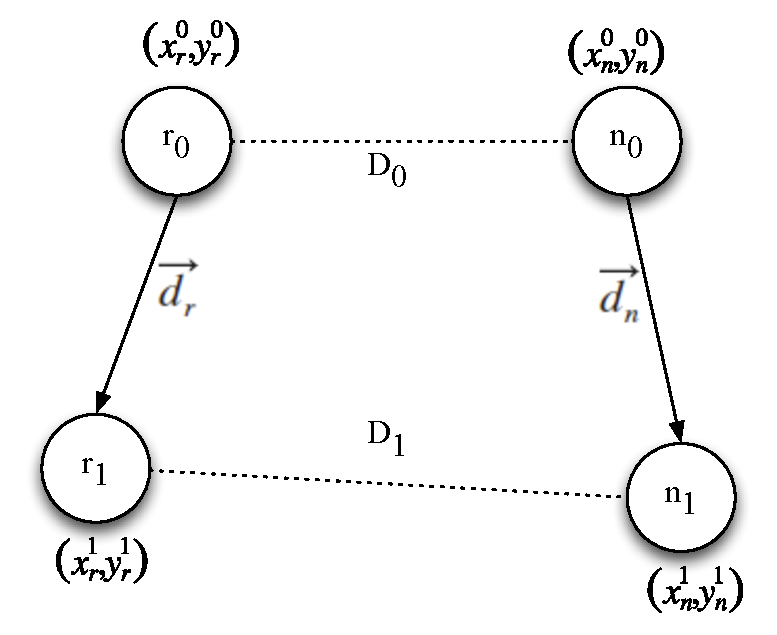
\includegraphics[width=4.5in]{Figures/NodeRankingModel.pdf}
\caption{Node ranking model}
\label{Node ranking model}
\end{figure}

%=============================================================================
\section{Evaluation}
\label{DORSI:Evaluation}
%=============================================================================
\begin{table}[!t]
		\renewcommand{\arraystretch}{1.3}
		\centering
		\begin{tabular}{|c|c|c|}
			\hline
			Parameters         & DORSI                  & Epidemic \\ \hline
			Operation Time     & \multicolumn{2}{|c|}{3600 Seconds }  \\ \hline
			Message Size       &           \multicolumn{2}{|c|}{500 KB - 5 MB}        \\ \hline
			Node Buffer        &              \multicolumn{2}{|c|}{1000 MB   }       \\ \hline
			Transmission Range &              \multicolumn{2}{|c|}{150 Meters  }        \\ \hline
			Transmission Speed &              \multicolumn{2}{|c|}{ 54 Mbps   }        \\ \hline
			Node Density       &                \multicolumn{2}{|c|}{0 - 100 \% }        \\ \hline
			Router             & DORSI                  & Epidemic \\ \hline
			Deadline                &  \multicolumn{2}{|c|}{Relative to data class}       \\ \hline
			Moving Speed       &          \multicolumn{2}{|c|}{0.5 - 1.5 m/s }        \\ \hline
			Movement Model     &       \multicolumn{2}{|c|}{Random Waypoint  }      \\ \hline
			Wait Time     &       \multicolumn{2}{|c|}{0 - 180 Seconds  }      \\ \hline
			Number of classes     &       \multicolumn{2}{|c|}{5 }      \\ \hline
		\end{tabular}
		\caption{DORSI Simulation variables}
		\label{TB:DORSI:table_parameters}
	\end{table}

\subsection{Simulation setup}
This protocol is designed to implement on any network that messages can be classified by data content. 
%%
We select the military tactical network as a sample application to present and evaluate this protocol because of its opportunistic behavior. 
%%
Since military tactical networks are subject to frequent disruption of end-to-end communication, current traditional network protocol tends to poorly handle these disruptive environment. 
%%
In this extreme scenario, opportunistic network with store-carry-forward scheme can be integrated into this tactical network to aid significant and secure operations. 
%%
In addition we employ MLS \cite{Winjum2008} as a classification of data in this military scenario environment, consisting of 5 classes.

We conduct the extensive simulations using the ONE 1.4.1 (The Opportunistic Network Environment simulator) \cite{Keranen2009b}. 
%%
ONE is a powerful JAVA tool for generating different movement models, running simulation with various routing protocols, visualizing simulations in real time and generating results, and post processing the results.

We implement new DORSI router with the designed simulation scenario to compare with modified traditional Epidemic routing protocol \cite{Vahdat2000}. 
%%
The Epidemic router is modified with the same classification as DORSI router in order to compare the actual performance between them. 
%%
However, the classification implemented in modified Epidemic router is not effected the message routing decision. 
%%
The Epidemic router treats every message the same while DORSI router routes messages differently according to their DORSI parameters. 
%%
Basically, the performance of opportunistic network correlates with the simulation parameters. 
%%
In our tactical network simulation environment, we implement the scenario corresponding to the actual military operation. 
%%
The common message in this tactical network traffic is usually commands in short message format, locations or images which the size of approximately 500 KB to 5 MB. 
%%
A mobile node is assumed to be a soldier equipped with modern communication equipment with transmission speed and range of 54 Mbps and 150 Meters respectively. 
%%
In addition, each node can hold up to 1 GB of storage for buffering the in-transmitted messages while randomly moving at a speed of 0.5 to 1.5 m/s. 
%%
The simulation time is set for 1 hour to study the behavior of messages inside the network traffic. 
%%
To evaluate the impact of message classification, we compare the performance of each router by varying the node density. 
%%
In random way point movement (RWP), nodes can move around in random zigzag paths. The nodes can move around randomly in a 1,000 m x 1,000 m area with walking speed. 
%%
In our experiment, the total number of nodes in a network per a one $km^2$ area denotes its node density. 
%%
Each message embedded with the deadline value correlative to the degree of that data sensitivity.

\subsection{Metric}
To evaluate DORSI with Epidemic routing protocol, we define two keys performance index corresponding to our design concept: Effective Delivery Ratio (EDR) and Effective Replication Ratio (ERR). 
%%
Our protocol disseminates the data by its degree of sensitivity, therefore in order to analyze actual performance this evaluation requires appending higher credential weight on the successful delivery of data with higher significant level. 
%%
Basically, delivery ratio is defined by the ratio of the total number of messages delivered to the total number of messages created. 
%%
In our evaluation, EDR can be computed by introducing significant level ($S_i$) into the number of delivered messages within the deadline ($M_d$) from each class to the number of created messages ($M_c$) as in equation \ref{Eq:DORSI:EDR}.

\begin{eqnarray}
\label{Eq:DORSI:EDR}
EDR=\frac { \sum _{ j=1 }^{ m }{ { S }_{ i }^{ j }{ M }_{ d }^{ j } }  }{ { M }_{ c }^{ j } } 
\end{eqnarray}

On the other hand, we can compute ERR by the number of replicated messages ($M_r$) that incorporate with security level ($S_e$) to the total created messages as in equation \ref{Eq:DORSI:ERR}. 
%%
The higher ERR means more message replicas in the network resulting in excessive network resource consumption and higher security risk.

\begin{eqnarray}
\label{Eq:DORSI:ERR}
ERR=\frac { \sum _{ j=1 }^{ m }{ { S }_{ e }^{ j }{ M }_{ r }^{ j } }  }{ { M }_{ c }^{ j } } 
\end{eqnarray}

%%%%%%%%%%%%%%%%%%%%%%%%%%%%%%%%%%%%%%%%%%%%%%%%%%%%%%%%%%%%%%%%%%%%
\subsection{Result}
%%%%%%%%%%%%%%%%%%%%%%%%%%%%%%%%%%%%%%%%%%%%%%%%%%%%%%%%%%%%%%%%%%%%

\begin{figure}[!h]
\centering
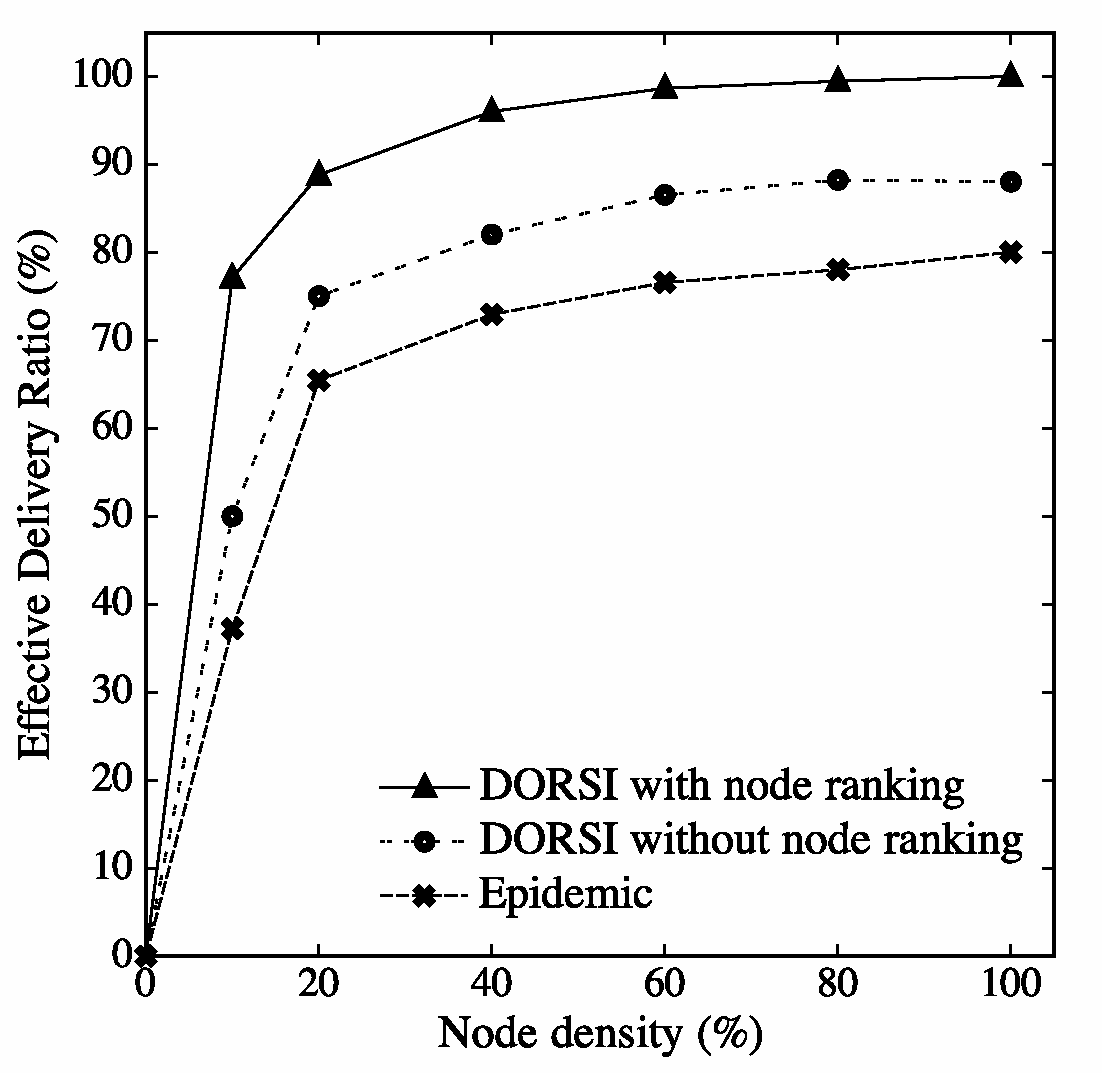
\includegraphics[width=3in]{Graphs/EDR_NodeDensity.pdf}
\caption{Effective Delivery Ratio comparison}
\label{Fig:DORSI:Effective Delivery Ratio comparison}
\end{figure}

Our implementation consists of two presenting keys: deliverable of significant data and security risk. 
%%
Firstly, we analyze the EDR value to determine the delivery guarantee for important data. 
%%
Figure \ref{Fig:DORSI:Effective Delivery Ratio comparison} presents the relationship between effective delivery ratio and node density comparing DORSI to epidemic routing. 
%%
This graph illustrates that DORSI gains remarkably higher EDR than the Epidemic, approximately 35\%. 
%%
By the common nature of flooding based routing, the EDR increases with the node density because node can obtain higher tendency of successful message delivery when the number of nodes increase. 
%%
In addition, at sparse node density condition (less than 10\%), the EDRs of 3 simulated routing protocols are similar because of our prioritization technique requires specific amount of nodes in order to efficiently perform. 
%%
Nevertheless, achieving 100\% EDR is impractical even though all resource is utilized for this purpose. 
%%
Message prioritization can improve the overall EDR about 10\% over epidemic while node ranking mechanism can increase approximately more 25\% EDR than DORSI without node ranking.

\begin{figure}[!h]
\centering
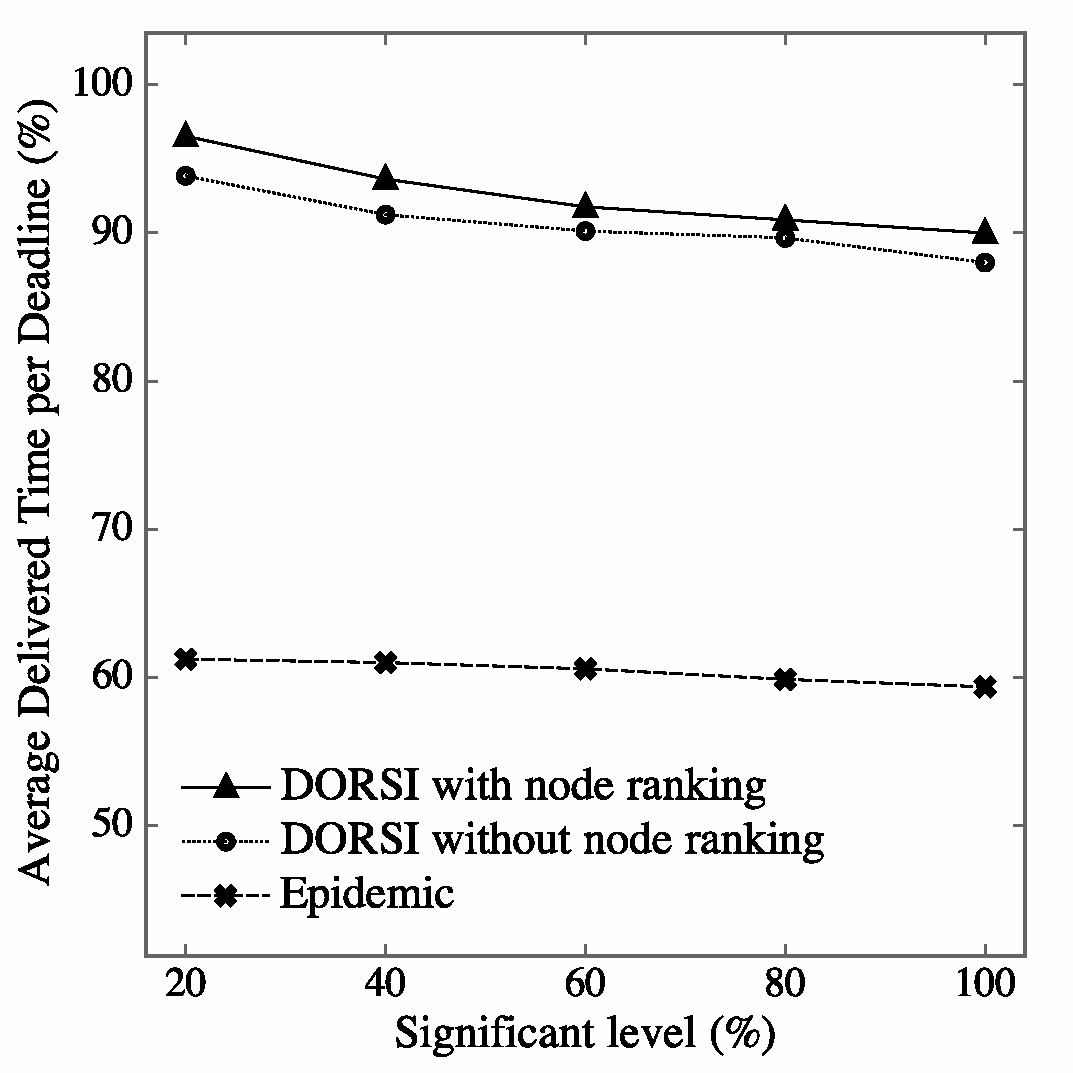
\includegraphics[width=3in]{Graphs/ADTD_significantLevel.pdf}
\caption{Average Delivered Time per Deadline on Significant Level}
\label{Fig:DORSI:Average Delivered Time per Deadline on Significant Level}
\end{figure}

As a result, DORSI outperforms Epidemic due to these design components: Firstly, by introducing deadline into our message prioritization method, the message with higher significant level can reach the destination faster. 
%%
This concept is supported by the Average Delivered Time (ADT) per deadline to significant level as shown in Fig. \ref{Fig:DORSI:Average Delivered Time per Deadline on Significant Level}. This graph presents that the messages routing with DORSI can reach the destination closer to their deadline than epidemic counterpart. 
%%
The consequence from Fig. \ref{Fig:DORSI:Effective Delivery Ratio comparison} and \ref{Fig:DORSI:Average Delivered Time per Deadline on Significant Level} shows that higher EDR of DORSI is a result from optimizing the time of delivery to their deadline.

\begin{figure}[!h]
\centering
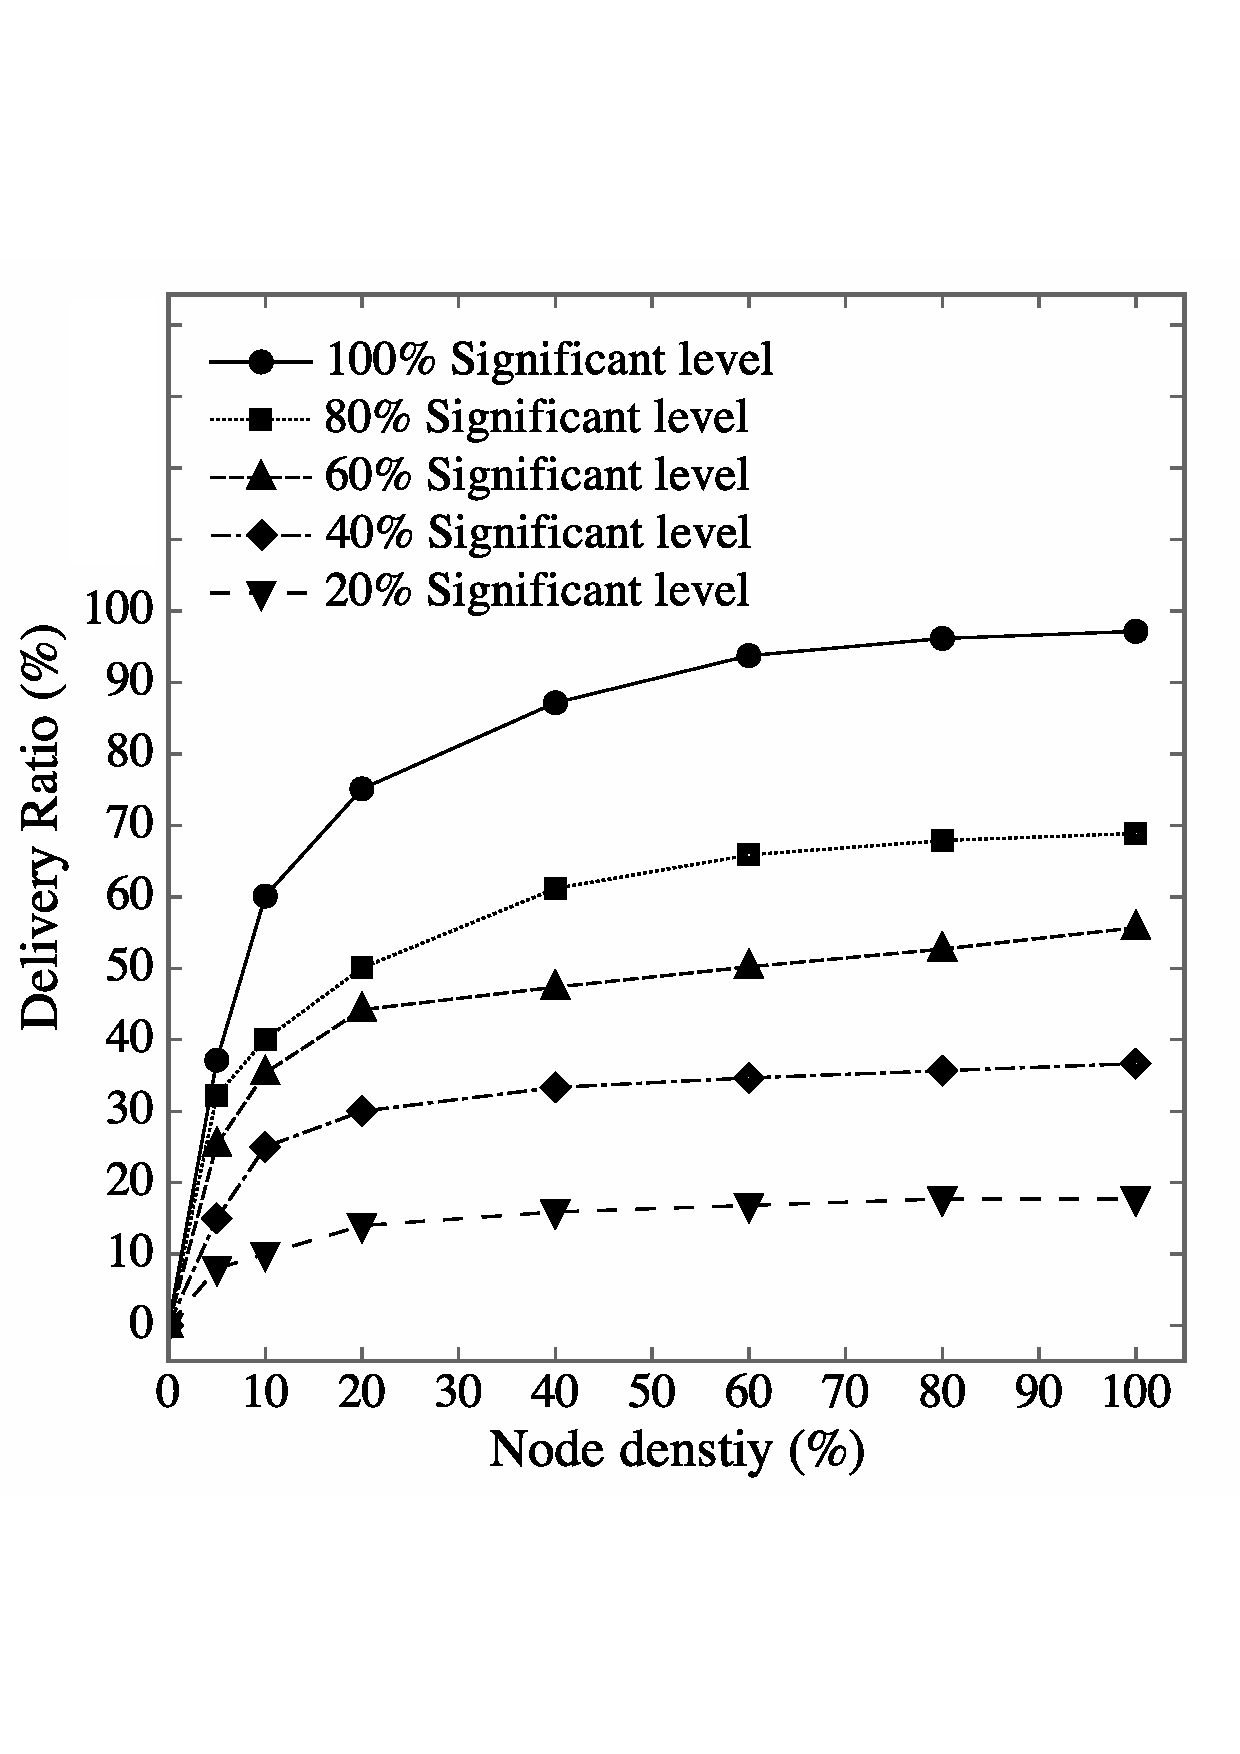
\includegraphics[width=3in]{Graphs/DR_NodeDenstiy2.pdf}
\caption{DORSI Delivery Ratio on each class}
\label{Fig:DORSI:DORSI Delivery Ratio on each class}
\end{figure}

Message prioritization technique can increase the delivery ratio of important data as in Fig. \ref{Fig:DORSI:DORSI Delivery Ratio on each class}. 
%%
This graph shows the relationship between delivery ratios of each class in DORSI to the node density. 
%%
Normally, messages with higher significant level (such as top secret or secret data) obtain more chance of successfully reaching the destination than others. The result clearly suggests that the delivery ratio of data with higher significant level is higher than less important data. 
%%
Comparing delivery ratio on each class of DORSI and Epidemic, the message prioritization can distinguish the significant level of messages. 
%%
On the other hand, the delivery ratio of all classes on Epidemic routing in Fig. \ref{Fig:DORSI:Epidemic Delivery Ratio on each class} are similar while the delivery ratio of DORSI increases by its classes. 
%%
Consequently, the message prioritization can control the delivery time of each class resulting in overall deliverable improvement.

\begin{figure}[!h]
\centering
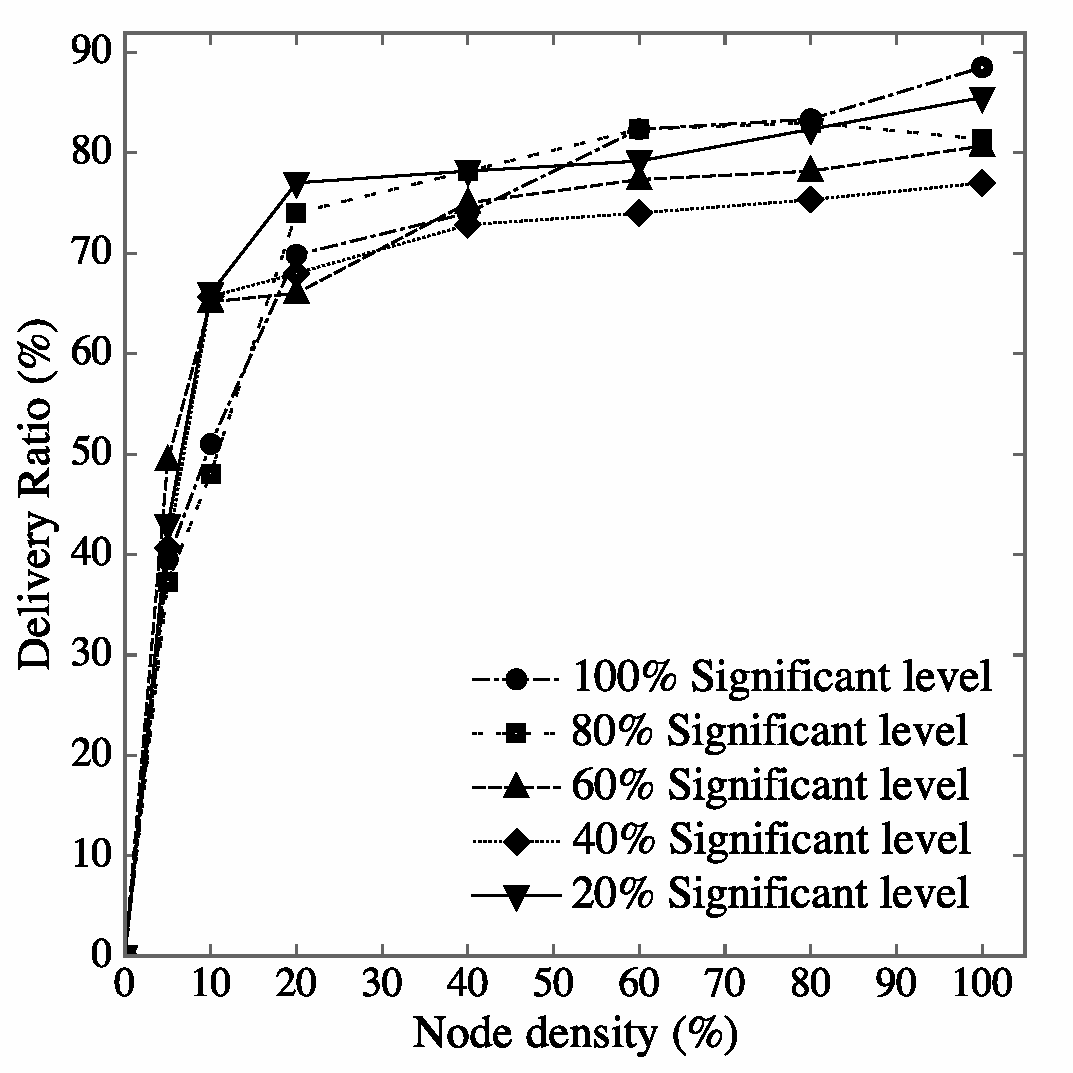
\includegraphics[width=3in]{Graphs/EpidemicDeliveryRatiooneachclass.pdf}
\caption{Epidemic Delivery Ratio on each class}
\label{Fig:DORSI:Epidemic Delivery Ratio on each class}
\end{figure}

Node ranking mechanism can enhance more EDR of DORSI over this same protocol without node ranking. 
%%
By selecting the best candidate nodes to transmit the data, the important messages can gain more chance of reaching the destination. 
%%
Fig. \ref{Fig:DORSI:Effective Delivery Ratio comparison} and \ref{Fig:DORSI:Effective Replication Ration Comparison} clearly shows that the node selecting technique can improve the performance of DORSI without node ranking. 
%%
This significantly benefits the network resource consumption and higher chance of deliverable of important data.

\begin{figure}[!h]
\centering
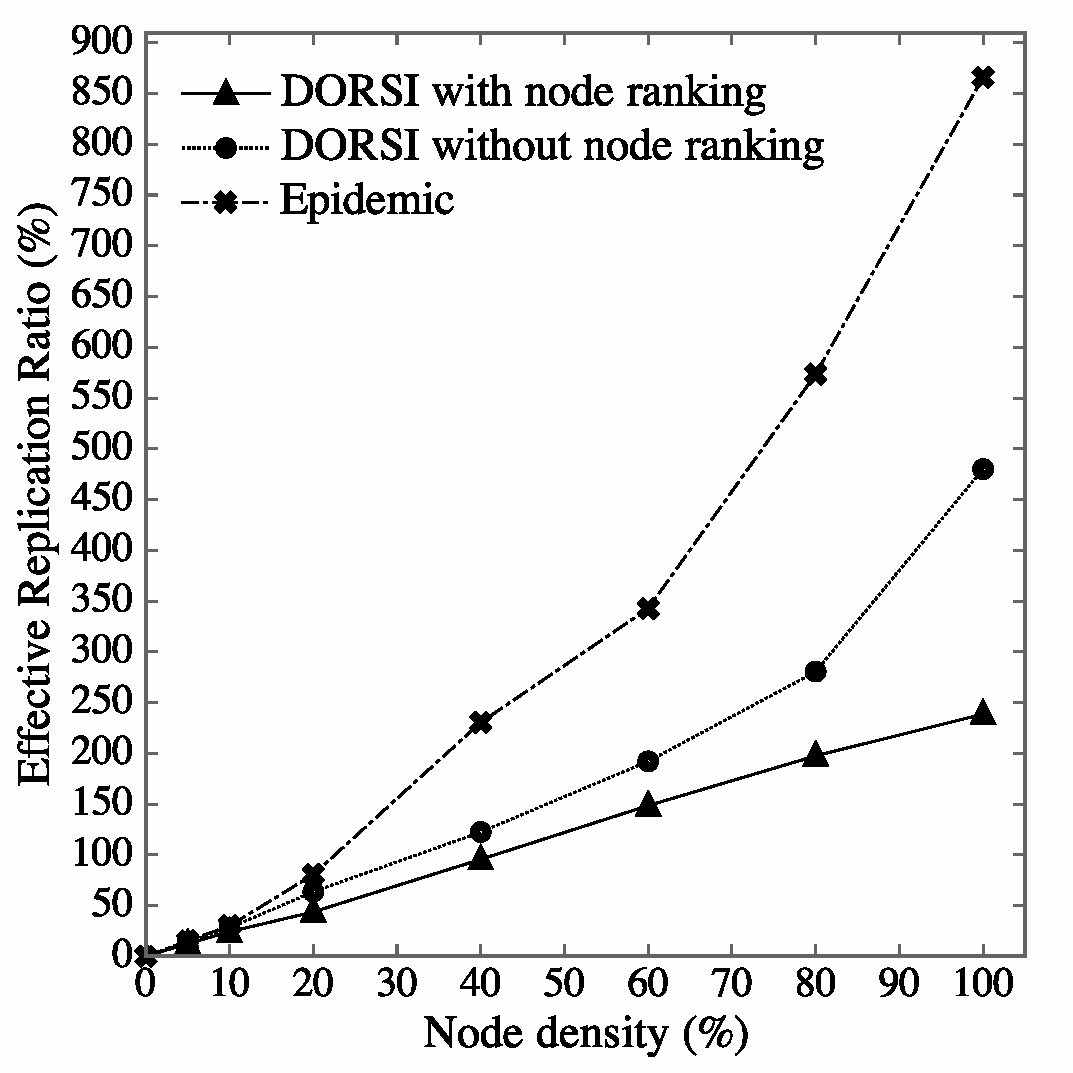
\includegraphics[width=3in]{Graphs/EffectiveReplicationRationComparison.pdf}
\caption{Effective Replication Ratio Comparison}
\label{Fig:DORSI:Effective Replication Ration Comparison}
\end{figure}

On the other hand, the ERR is analyzed to assess the security risk. 
%%
The ERR of Epidemic and DORSI without node ranking exponentially increase while DORSI with node ranking gradually rises as in Fig. \ref{Fig:DORSI:Effective Replication Ration Comparison}. 
%%
This graph shows the relationship between effective replication ratio and node density. 
%%
The lower number of ERR means that less message replicas in the network resulting in less security risk. 
%%
Because the DORSI protocol can efficiently control the number of message replication in the network traffic, the number of message copies are remarkably lower than Epidemic. 
%%
This result proves our design concept of security risk and aids in the optimum network bandwidth utilization.

To study the behavior of our protocol, we analyze the result of various number of classes as well. 
%%
In our scenario, we divide the data class based on British MLS scheme with 5 level of security: Top Secret (T), Secret (S), Restrict (R), Confidential (C) and Unclassified (U). 
%%
However, there are other MLS schemes for different zone of military, for example, the US. 
%%
DoD employs only 4 level of security: T, S, C and U. In order to deploy our method to different class of data, we simulate the data with different scale of classes. 
%%
Fig. \ref{Fig:DORSI:EDR on different classification scale} shows the comparison of effective delivery ratio and node density between different class scales from 1 to 5 classes. 
%%
This graph shows the similar trend between all classes which is the more node density the higher the delivery ratio. 
%%
The overall EDR increases when the messages are classified with more number of classes. 
%%
This is the outcome from DORSI routing which requires some node amount to process the node ranking mechanism. 
%%
This result proves that the classification technique can be deployed to various number of classes in any application.

\begin{figure}[!h]
\centering
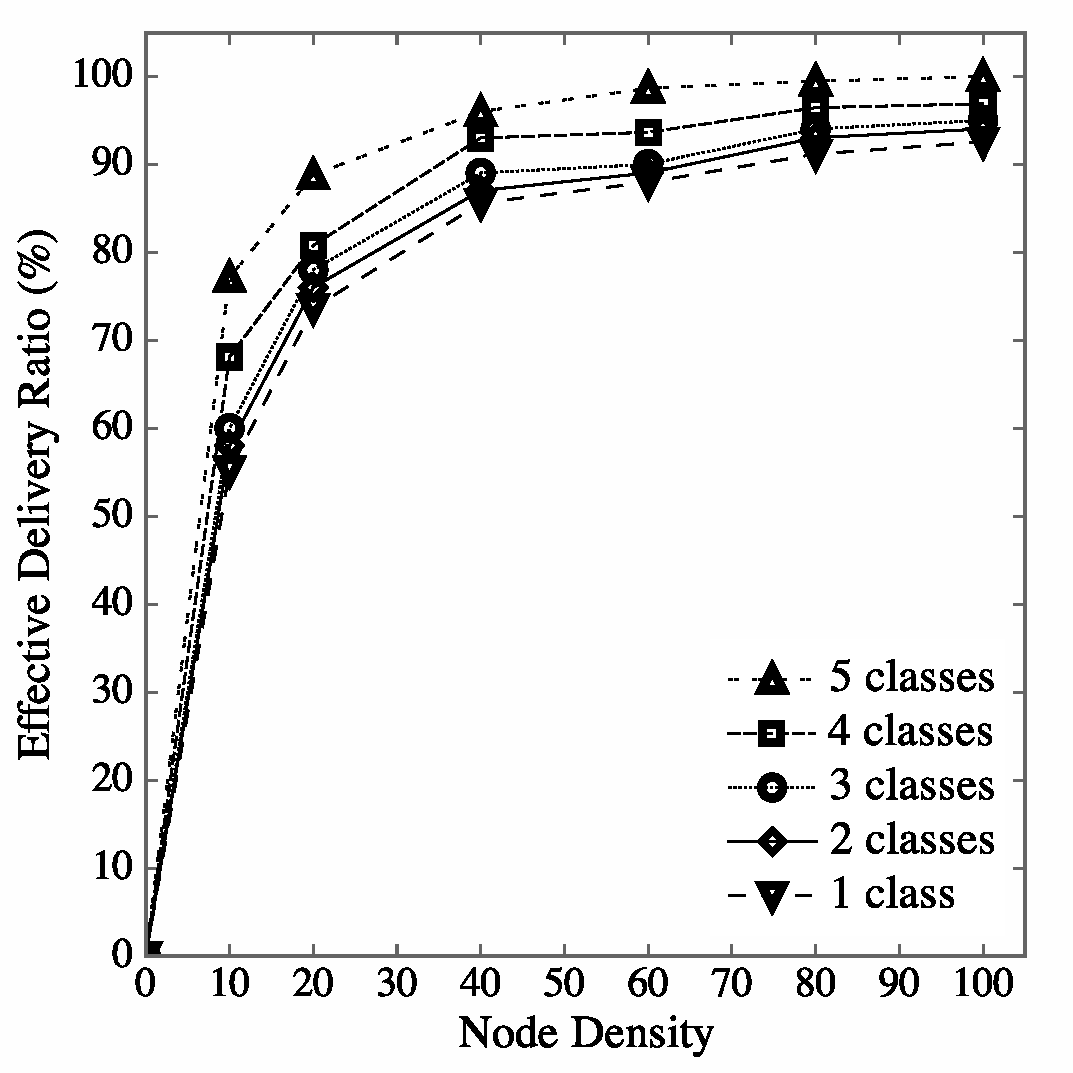
\includegraphics[width=3in]{Graphs/EDRondifferentclassificationscale.pdf}
\caption{EDR on different classification scale}
\label{Fig:DORSI:EDR on different classification scale}
\end{figure}

To study the behavior of DORSI, we select 20\% node density scenario aiming to analyze its performance by varying the transmission range of simulation parameters. 
%%
Fig. \ref{Fig:DORSI:EDR comparing varied by transmission range} presents the relationship of EDR to the node transmission range. 
%%
The result shows that the EDR increase with transmission range especially after 50 meters. 
%%
However after the range of 150 meters, the EDR tends to slightly decline. 
%%
By increasing the transmission range, transmitting node in DORSI can increase its opportunity to selecting the candidate nodes, resulting in more chance of reaching destination.

\begin{figure}[!h]
\centering
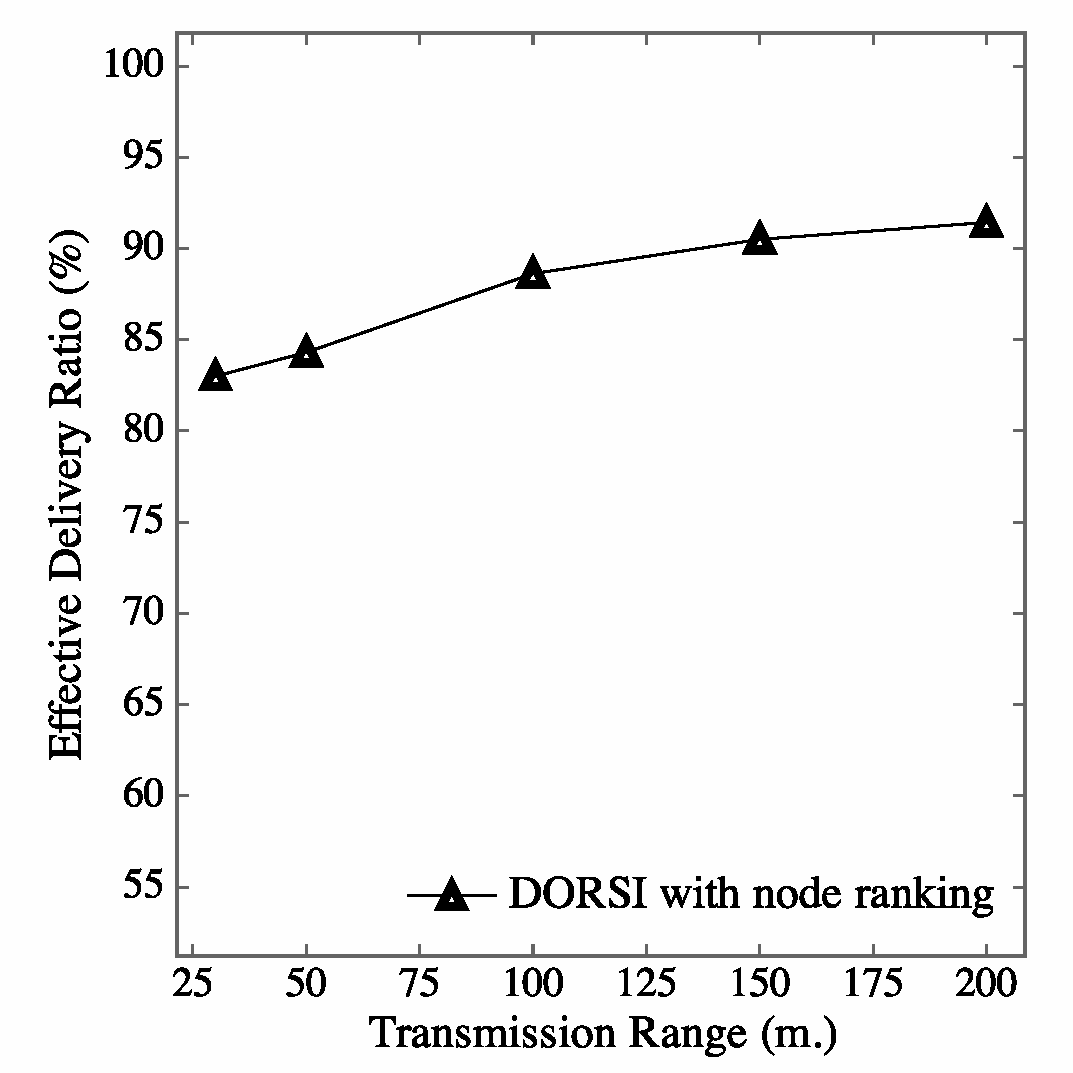
\includegraphics[width=3in]{Graphs/EDRcomparingvariedbytransmissionrange.pdf}
\caption{EDR comparing varied by transmission range}
\label{Fig:DORSI:EDR comparing varied by transmission range}
\end{figure}

All in all, the key performance from simulation results confirms with our design goals. 
%%
In DORSI, the value of EDR and ERR shows that we can control the message replication thus the message with higher priority can reach the destination faster to prove the concept of significant level and security level. 
%%
In addition, the value of ADT proves that we can control the messages to reach the destination near their expiration. 
%%
Normally, the delivery ratio increases with the number of message copies.
%%
However, our approach can maintain the delivery ratio while reducing the message replicas in the network. 
%%
As a result, this method significantly optimizes the network utilization. 
%%
The drawback of this protocol is high processing time since these executable nodes require amount of computation time.

%=============================================================================
\section{Conclusion}
\label{DORSI:Conclusion}
%=============================================================================
In this chapter, we propose a novel Data-wise Opportunistic Routing with Spatial Information (DORSI) in order to classify the messages based on the information sensitivity concept along with nodes prioritization technique corresponding to the their delivery probability computed by spatial data. 
%%
This protocol classifies the messages according to their significant level, security level and deadline relative to the sensitivity level of data. 
%%
Meanwhile, this chapter adapts the geographical routing technique to select the best candidate node to forward the messages to the destination. 
%%
Simulation experiments clearly illustrate that two key performance indexes — effective delivery ratio and effective replication ratio — remarkably improve over the traditional Epidemic routing. Moreover, the delivery ratio of DORSI and Epidemic comparison shows notable overall enhancement of the network routing efficiency. 
%%
This means that DORSI protocol can guarantee higher delivery ratio on more important data while limiting the replication of data with higher security level. 
%%
The average delivered time of DORSI also shows the optimal bandwidth utilization since it can control the messages to reach the destination closer to their deadline. 
%%
In addition, this method can be applied to different scale of data classification to suit any application deployment. 
%%
Furthermore, our work can be extended in various directions. 
%5
An obvious extension of the work could be the evaluation of our approach on a virtualization network to physically obtain the real life results comparing to the results from this simulation result. 
%%
Next, we will evaluate the performance of our method in different conditions in order to apply data classification routing technique on more general applications.
%%











































